% !TEX root = task-1-8-2.tex
% Editable task bank. Append new BankTask blocks at the end of the document.
\documentclass[12pt,a4paper]{article}
\usepackage{physics-textbook}
\usepackage{graphicx,needspace}
\usetikzlibrary{decorations.pathmorphing}
\newif\ifShowSolutions
\ifdefined\TutorEdition
  \ShowSolutionstrue
\else
  \ShowSolutionsfalse % Change to \ShowSolutionstrue to display solutions.
\fi
\newcounter{banktask}
\newsavebox{\BankTaskBox}
\newcommand{\BankTaskContent}[3]{%
  \noindent\textbf{\thebanktask.}\quad #2\par
  \ifShowSolutions
    \Needspace{50mm}% Keep the solution heading with its opening text or diagram.
    #3\par
    \ifdefined\TutorEdition
      \ifcsname TutorSource#1\endcsname
        \nopagebreak\smallskip{\small\csname TutorSource#1\endcsname\par}%
      \fi
    \fi
  \fi
}
\newcommand{\BankTask}[3]{%
  \refstepcounter{banktask}\par\medskip
  \sbox{\BankTaskBox}{\begin{minipage}{\linewidth}%
    \BankTaskContent{#1}{#2}{#3}\end{minipage}}%
  \ifdim\dimexpr\ht\BankTaskBox+\dp\BankTaskBox\relax>\dimexpr\textheight-20mm\relax
    \Needspace{35mm}\BankTaskContent{#1}{#2}{#3}%
  \else
    \Needspace{\dimexpr\ht\BankTaskBox+\dp\BankTaskBox\relax}%
    \noindent\usebox{\BankTaskBox}\par
  \fi
  \medskip
}
\begin{document}
\BookSubsection{1.8.2}{Второй закон Ньютона}


% Source sdamgia-312: https://phys-ege.sdamgia.ru/problem?id=312
\BankTask{sdamgia-312}{
Под действием одной силы $F_{1}$ тело движется с ускорением $4\,\text{м/с}^{2}$. Под действием другой силы $F_{2}$, направленной противоположно силе $F_{1}$, ускорение тела равно $3\,\text{м/с}^{2}$. С каким ускорением тело будет двигаться при одновременном действии сил $F_{1}$ и $F_{2}$? Ответ дайте в метрах на секунду в квадрате.
}{
\smallskip\noindent\textbf{Решение}\par
Согласно второму закону Ньютона, ускорение тела пропорционально равнодействующей всех сил, действующих на него: $F_{\text{равн}}=ma,$ $F_1=ma_1,$ $F_2=ma_2.$ Силы $F_1$ и $F_2,$ по условию, направлены противоположно, поэтому при их одновременном действии тело будет двигаться с ускорением: 

\[a= \frac{F_{\text{равн}}}{m} = \frac{F_1 - F_2}{m} =a_1 - a_2=4\,\text{м/с} ^2 - 3\,\text{м/с} ^2 =1\,\text{м/с} ^2 .\]

Ответ: $1$.
}

% Source sdamgia-3469: https://phys-ege.sdamgia.ru/problem?id=3469
\BankTask{sdamgia-3469}{
На полу лифта, разгоняющегося вверх с постоянным ускорением $a=1\,\text{м/с} ^2 ,$ лежит груз массой $5\,\text{кг}$. Каков вес этого груза? Ответ выразите в ньютонах.
}{
\smallskip\noindent\textbf{Решение}\par
Весом $\vec P$ называется сила, с которой тело давит на опору или растягивает подвес. По третьему закону Ньютона эта сила равна по величине и противоположна по направлению силе реакции опоры $\vec N.$ Поэтому определим последнюю, для того чтобы вычислить вес тела в лифте. Для этого выпишем второй закон Ньютона для тела в проекции на вертикальную ось, направленную вверх. Груз движется вместе с лифтом вверх с ускорением $a$, на него действует две силы: сила тяжести и искомая сила реакции опоры:

\[ma=N - mg \Longleftrightarrow  N=m ( g + a ) .\]

Следовательно, вес тела равен:

\[P=m ( g + a ) =5 \cdot  ( 10 + 1 ) =55\,\text{Н}.\]

Ответ: $55$.
}

% Source sdamgia-10174: https://phys-ege.sdamgia.ru/problem?id=10174
\BankTask{sdamgia-10174}{
Тело массой $2\,\text{кг}$ лежит на гладкой горизонтальной плоскости. В момент времени $t = 0$ к этому телу прикладывают две взаимно перпендикулярные силы $\vec F_1$ и $\vec F_2,$ направленные горизонтально, модули которых изменяются со временем $t$ по законам $F_1=3t$ и $F_2=4t,$ а направления не меняются. Определите модуль ускорения тела в момент времени $t = 4\,\text{с}$. Ответ выразите в метрах на секунду в квадрате.
}{
\smallskip\noindent\textbf{Решение}\par
Так как силы перпендикулярны друг другу, то их равнодействующая будет равна:

\[F= \sqrt{F_1 ^2 + F_2 ^2} =5t.\]

По второму закону Ньютона в момент времени $t = 4\,\text{с}$ тело будет двигаться с ускорением, равным по модулю:

\[a= \frac{F}{m} = \frac{5 \cdot  4}{2} =10\,\text{м/с} ^2 .\]

Ответ: $10$.
}

% Source sdamgia-10215: https://phys-ege.sdamgia.ru/problem?id=10215
\BankTask{sdamgia-10215}{
На шероховатой горизонтальной поверхности находится тело массой $3\,\text{кг}$. К нему приложена горизонтально направленная сила, модуль которой равен $8\,\text{Н}$. Коэффициент трения между поверхностью и телом равен $0{,}2$. Модуль приложенной к телу силы увеличивают до $10\,\text{Н}$, не изменяя ее направления.

Как изменятся в результате этого модуль ускорения тела и модуль действующей на тело силы трения?

Для каждой величины определите соответствующий характер изменения.

$1$. Увеличится.

$2$. Уменьшится.

$3$. Не изменится.

 

\begin{center}\small\renewcommand{\arraystretch}{1.25}\begin{tabular}{|p{0.450\linewidth}|p{0.450\linewidth}|}\hline
Модуль ускорения тела & Модуль действующей на тело силы трения\\\hline
 & \\\hline
\end{tabular}\end{center}
}{
\smallskip\noindent\textbf{Решение}\par
При условии, что тело движется, на него будет действовать сила трения, равная:

\[F_{\text{тр}}=\mu N=\mu mg=6\,\text{Н},\]

где $N$ — сила реакции опоры. Поскольку сила трения меньше приложенной силы в $8\,\text{Н}$, то тело движется с ускорением. Увеличение модуля приложенной силы приведет к увеличению модуля ускорения.

Поскольку тело изначально двигалось, то сила трения не изменится.

Ответ: $13$.
}

% Source sdamgia-19659: https://phys-ege.sdamgia.ru/problem?id=19659
\BankTask{sdamgia-19659}{
Камень бросили вертикально вверх при наличии сопротивления воздуха. Во время своего полета камень проходит некоторую точку $A$ дважды — первый раз при движении вверх, а во второй раз — при движении вниз. Как изменяются модуль ускорения камня и модуль скорости камня при втором прохождении через точку $A$ по сравнению с первым прохождением через эту точку? 

Для каждой величины определите соответствующий характер ее изменения.

$1$. Увеличивается.

$2$. Уменьшается.

$3$. Не изменяется.

 

\begin{center}\small\renewcommand{\arraystretch}{1.25}\begin{tabular}{|p{0.450\linewidth}|p{0.450\linewidth}|}\hline
Модуль ускорения & Модуль скорости\\\hline
 & \\\hline
\end{tabular}\end{center}
}{
\smallskip\noindent\textbf{Решение}\par
$1$. Модуль ускорения. 

При движении камня вверх: по второму закону Ньютона $ma_1y = - mg - F_{\text{сопр}},$ откуда $a_1y = - g - \frac{F_{\text{сопр}}}{m} ,$ $|a_1| = g + \frac{F_{\text{сопр}}}{m} .$ При движении камня вниз: $ma_2y= - mg + F_{\text{сопр}},$ откуда $a_2y = - g + \frac{F_{\text{сопр}}}{m} ,$ $|a_2| = - g + \frac{F_{\text{сопр}}}{m} .$ Следовательно, модуль ускорения уменьшается.

$2$. Модуль скорости. 

Полная энергия из-за действия силы сопротивления уменьшается. Поэтому при повторном прохождении точки А кинетическая энергия камня уменьшится и, соответственно, уменьшится его скорость. 

Ответ: $22$.
}

% Source sdamgia-19882: https://phys-ege.sdamgia.ru/problem?id=19882
\BankTask{sdamgia-19882}{
На тело массой $2\,\text{кг}$ действует сила $60\,\text{Н}$. Найдите ускорение тела. Ответ дайте в метрах на секунду в квадрате.
}{
\smallskip\noindent\textbf{Решение}\par
По второму закону Ньютона: 

\[a= \frac{F}{m} = \frac{60}{2} =30 \frac{\text{м}}{\text{с} ^2} .\]

Ответ: $30$.
}

% Source sdamgia-28080: https://phys-ege.sdamgia.ru/problem?id=28080
\BankTask{sdamgia-28080}{
Мальчик поднимает вверх гирю массой $12\,\text{кг}$, действуя на нее постоянной силой $140\,\text{Н}$, направленной вертикально вверх. 

$1$. Если мальчик приложит к гире направленную вертикально сила $100\,\text{Н}$, он не сможет ее поднять.

$2$. Гиря действует на руку мальчика с силой $100\,\text{Н}$, направленной вниз.

$3$. Вес гири равен $140\,\text{Н}$ и направлен вверх.

$4$. Равнодействующая сил, действующих на гирю, равна $20\,\text{Н}$ и направлена вверх.

$5$. Ускорение гири равно $2\,\text{м/с}^{2}$.
}{
\smallskip\noindent\textbf{Решение}\par
$1$. Верно. Сила тяжести, действующая на гирю, равна $F_=mg=12 \cdot  10\,\text{м/с} ^2 =120\,\text{Н}.$ Если мальчик приложит силу $100\,\text{Н}$, то не сможет поднять гирю. 

$2$. Неверно. По третьему закону Ньютона сила, с которой гиря действует на руку мальчика, равна силе, с которой мальчик действует на нее, то есть $140\,\text{Н}$. 

$3$. Неверно. Вес гири направлен вниз. 

$4$. Верно. Модуль равнодействующей сил, направленных в противоположные стороны, равен разности модулей этих сил, то есть $140 - 120 = 20\,\text{Н}$. 

$5$. Неверно. По второму закону Ньютона для равнодействующей силы:

\[a= \frac{F}{m} = \frac{20\,\text{Н}}{12\,\text{кг}} \approx1{,}7\,\text{м/с} ^2 .\]

Ответ: $14$.
}

% Source sdamgia-29442: https://phys-ege.sdamgia.ru/problem?id=29442
\BankTask{sdamgia-29442}{
В лаборатории исследовали прямолинейное движение тела массой $m = 300\,\text{г}$ из состояния покоя. В таблице приведена экспериментально полученная зависимость пути, пройденного телом, от времени.  

\begin{center}\small\renewcommand{\arraystretch}{1.25}\begin{tabular}{|c|c|c|c|c|c|c|c|c|}\hline
$t$, с & $0$ & $1$ & $2$ & $3$ & $4$ & $5$ & $6$ & $7$\\\hline
$L$, м & $0$ & $1$ & $4$ & $9$ & $16$ & $25$ & $36$ & $49$\\\hline
\end{tabular}\end{center}

$1$. Тело двигалось равноускоренно.

$2$. Скорость тела в момент времени $4\,\text{с}$ равнялась $8\,\text{м/с}$.

$3$. Кинетическая энергия тела в момент времени $5\,\text{с}$ равна $25\,\text{Дж}$.

$4$. Равнодействующая сил, действующих на тело, все время возрастала.

$5$. За первые $3\,\text{с}$ работа равнодействующей сил, действующих на тело, была равна $5{,}4\,\text{Дж}$.
}{
\smallskip\noindent\textbf{Решение}\par
$1$. Верно. При движении тела из состояния покоя зависимость пути от времени имеет вид $L\sim t ^2 .$ 

$2$. Верно. Из формулы прямолинейного равноускоренного движения из состояния покоя $L= \frac{v t}{2}$ следует, что скорость:

\[v = \frac{2L}{t} = \frac{2 \cdot  16}{4} =8\,\text{м/с}.\]

$3$. Неверно. Аналогично предыдущему пункту найдем скорость тела в момент времени $5\,\text{с}$: 

\[v = \frac{2L}{t} = \frac{2 \cdot  25}{5} =10\,\text{м/с}.\]

Тогда кинетическая энергия тела в этот момент времени равна:

\[E_k= \frac{m v ^2}{2} = \frac{0{,}3 \cdot  10 ^2}{2} =15\,\text{Дж}.\]

$4$. Неверно. Движение равноускоренное, с постоянным ускорением. Из второго закона Ньютона следует, что равнодействующая сил, действующих на тело, также будет постоянной. 

$5$. Верно. По теореме о кинетической энергии $A=\Delta E_k=E_k$ (с учетом, что начальная скорость равна $0$). Скорость тела в момент времени $3\,\text{с}$ равна:

\[v = \frac{2L}{t} = \frac{2 \cdot  9}{3} =6\,\text{м/с},\]

 а кинетическая энергия:

\[E_k= \frac{m v ^2}{2} = \frac{0{,}3 \cdot  6 ^2}{2} =5{,}4\,\text{Дж}.\]

Таким образом, работа за первые $3\,\text{с}$ равнодействующей сил равна $5{,}4\,\text{Дж}$.

Ответ: $125$.
}

% Source sdamgia-33062: https://phys-ege.sdamgia.ru/problem?id=33062
\BankTask{sdamgia-33062}{
K потолку лифта прикреплена пружина жесткостью $100$ H/м, к пружине прикрепили груз некоторой массы. Лифт начинает движение вниз с ускорением $2{,}5\,\text{м}$/$c^{2}$. Найдите массу груза, если удлинение пружин в состоянии покоя в движущемся лифте равно $1{,}5\,\text{см}$?
}{
\smallskip\noindent\textbf{Решение}\par
Когда лифт покоился, на груз действовали сила тяжести mg и сила упругости пружины, равная по закону Гука $F_{\text{упр}} = kx.$ Груз находился в покое, поэтому выполнялось равенство $mg = kx.$ При движении лифта вниз груз покоится относительно лифта, поэтому по второму закону Ньютона получаем:

\[ma = mg - F_{\text{упр}},\]

\[ma = mg - kx.\]

 Следовательно, масса груза равна

\[m = \frac{kx}{g - a} = \frac{100 \cdot  0{,}015}{10 - 2{,}5} = 0{,}2\,\text{кг}.\]

Ответ: $0{,}2\,\text{кг}$.
}

% Source sdamgia-38856: https://phys-ege.sdamgia.ru/problem?id=38856
\BankTask{sdamgia-38856}{
Груз массой $400\,\text{г}$ подвешен на пружине жесткостью $250\,\text{Н}$/м к потолку неподвижного лифта. Лифт равноускоренно опускается вниз в течение $3\,\text{с}$. На какое расстояние опускается лифт, если удлинение пружины при установившемся движении груза равно $1{,}5\,\text{см}$?
}{
\smallskip\noindent\textbf{Решение}\par
На груз действуют сила тяжести mg, направленная вертикально вниз, и сила упругости, равная по закону Гука $F_{\text{упр}} = kx$ и направленная вертикально вверх. При равноускоренном движении вниз по второму закону Ньютона получаем:

\[m \vec g + \overrightarrow F_{\text{упр}} = m \vec a,\]

\[Oy: mg - F_{\text{упр}} = ma.\]

 Таким образом, ускорение лифта равно $a = \frac{mg - kx}{m} .$ При равноускоренном движении без начальной скорости $s = \frac{at ^2}{2} .$ В результате находим:

\[s = \frac{( mg - kx ) t ^2}{2m} = \frac{( 0{,}4 \cdot  10 - 250 \cdot  0{,}015 ) \cdot  9}{2 \cdot  0{,}4} \approx 2{,}8\,\text{м}.\]

Ответ: $s \approx 2{,}8\,\text{м}.$
}


% Source 19F564: https://ege.fipi.ru/bank/questions.php?search=1&proj=BA1F39653304A5B041B656915DC36B38&qid=19F564
\BankTask{19F564}{
В инерциальной системе отсчёта некоторая сила сообщает телу массой $5\,\text{кг}$ ускорение, равное по модулю $3\,\text{м}/\text{с}^{2}$. Определите модуль ускорения, которое сообщит та же сила в той же системе отсчёта телу массой $7{,}5\,\text{кг}$ (в $\text{м}/\text{с}^{2}$).
}{
\smallskip\noindent\textbf{Решение от GPT}\par
По второму закону Ньютона $F=m_1a_1=m_2a_2$. Тогда\[a_2=\frac{m_1a_1}{m_2}=\frac{5\cdot3}{7{,}5}=2\,\text{м}/\text{с}^{2}.\] Ответ: $2$.
}

% Source 89A46D: https://ege.fipi.ru/bank/questions.php?search=1&proj=BA1F39653304A5B041B656915DC36B38&qid=89A46D
\BankTask{89A46D}{
Груз массой $200\,\text{г}$ подвешен на пружине к потолку неподвижного лифта. Лифт начинает двигаться и в течение $2\,\text{с}$ равноускоренно опускается вниз на расстояние $5\,\text{м}$. Каково удлинение пружины при опускании лифта, если её жёсткость $100\,\text{Н}/\text{м}$? Движение груза также считать равноускоренным, возникновением колебаний пренебречь. Удлинение выразите в $\text{см}$.
}{
\smallskip\noindent\textbf{Решение от GPT}\par
Лифт начинает движение из состояния покоя, поэтому $a=2s/t^2=2\cdot5/2^2=2{,}5\,\text{м}/\text{с}^{2}$. Ускорение направлено вниз. При $g=10\,\text{м}/\text{с}^{2}$ по второму закону Ньютона $mg-kx=ma$. Тогда\[x=\frac{m(g-a)}{k}=\frac{0{,}2(10-2{,}5)}{100}=0{,}015\,\text{м}=1{,}5\,\text{см}.\] Ответ: $1{,}5$.
}

% Source 2cB64F: https://ege.fipi.ru/bank/questions.php?search=1&proj=BA1F39653304A5B041B656915DC36B38&qid=2cB64F
\BankTask{2cB64F}{
В инерциальной системе отсчёта сила $\vec{F}$ сообщает телу массой $m$
ускорение, модуль которого равен $0{,}6\,\text{м}/\text{с}^{2}$. Чему равен модуль ускорения тела массой $2m$ под действием силы $\frac{1}{2}\vec{F}$ в этой системе отсчёта? Результат выразите в $\text{м}/\text{с}^2$.
}{
\smallskip\noindent\textbf{Решение от GPT}\par
$a_2/a_1=(F_2/F_1)(m_1/m_2)=1/4$, поэтому $a_2=0{,}6/4=0{,}15\,\text{м}/\text{с}^2$.
}

% Source 2622F3: https://ege.fipi.ru/bank/questions.php?search=1&proj=BA1F39653304A5B041B656915DC36B38&qid=2622F3
\BankTask{2622F3}{
В инерциальной системе отсчёта сила, равная по модулю $16\,\text{Н}$, сообщает телу массой $m$ ускорение $\vec{a}.$ Чему равен модуль силы, под действием которой тело массой $\frac{m}{2}$ будет иметь в этой системе отсчёта ускорение $\frac{\vec{a}}{4}?$ Результат выразите в $\text{Н}$.
}{
\smallskip\noindent\textbf{Решение от GPT}\par
$F_2/F_1=(m_2/m_1)(a_2/a_1)=1/8$. Отсюда $F_2=16/8=2\,\text{Н}$.
}

% Source 41AB52: https://ege.fipi.ru/bank/questions.php?search=1&proj=BA1F39653304A5B041B656915DC36B38&qid=41AB52
\BankTask{41AB52}{
В инерциальной системе отсчёта сила величиной $9\,\text{Н}$ сообщает телу
массой $3\,\text{кг}$ ускорение $\vec{a}.$ Какой должна быть масса тела, чтобы сила, равная $18\,\text{Н}$, сообщала ему в той же системе отсчёта ускорение $4 \vec{a}?$ Результат выразите в $\text{кг}$.
}{
\smallskip\noindent\textbf{Решение от GPT}\par
$a=9/3=3\,\text{м}/\text{с}^2$. Тогда $m_2=18/(4a)=1{,}5\,\text{кг}$.
}

% Source EC6256: https://ege.fipi.ru/bank/questions.php?search=1&proj=BA1F39653304A5B041B656915DC36B38&qid=EC6256
\BankTask{EC6256}{
В инерциальной системе отсчёта сила $\vec{F}$ сообщает телу массой $m$ ускорение $\vec{a}.$ Во сколько раз нужно уменьшить массу тела, чтобы вдвое меньшая сила сообщала ему в той же системе отсчёта в $3$ раза большее ускорение?
}{
\smallskip\noindent\textbf{Решение от GPT}\par
$m_2/m_1=(F_2/F_1)/(a_2/a_1)=(1/2)/3=1/6$. Массу нужно уменьшить в $6$ раз.
}

% Source 19872D: https://ege.fipi.ru/bank/questions.php?search=1&proj=BA1F39653304A5B041B656915DC36B38&qid=19872D
\BankTask{19872D}{
В инерциальной системе отсчёта сила величиной $70\,\text{Н}$ сообщает телу массой $10\,\text{кг}$ некоторое ускорение. Сила какой величины сообщит телу массой $9\,\text{кг}$ в этой же системе отсчёта такое же ускорение? Результат выразите в $\text{Н}$.
}{
\smallskip\noindent\textbf{Решение от GPT}\par
В первом случае $a=F_1/m_1=70/10=7\,\text{м}/\text{с}^2$. При том же ускорении $F_2=m_2a=9\cdot7=63\,\text{Н}$.
}

% Source 64F9A6: https://ege.fipi.ru/bank/questions.php?search=1&proj=BA1F39653304A5B041B656915DC36B38&qid=64F9A6
\BankTask{64F9A6}{
В инерциальной системе отсчёта сила, модуль которой равен $100\,\text{Н}$, сообщает некоторому телу ускорение $10\,\text{м}/\text{с}^{2}$. Каков модуль силы, которая сообщит этому телу ускорение $7\,\text{м}/\text{с}^{2}$ в этой системе отсчёта? Результат выразите в $\text{Н}$.
}{
\smallskip\noindent\textbf{Решение от GPT}\par
Масса $m=F_1/a_1=100/10=10\,\text{кг}$. Следовательно, $F_2=ma_2=10\cdot7=70\,\text{Н}$.
}

% Source A7Be77: https://ege.fipi.ru/bank/questions.php?search=1&proj=BA1F39653304A5B041B656915DC36B38&qid=A7Be77
\BankTask{A7Be77}{
В лабораторной работе изучали движение небольшого бруска массой $200\,\text{г}$ по горизонтальной шероховатой поверхности под действием горизонтальной постоянной силы, равной по модулю $800\,\text{мН}$. Зависимость модуля скорости бруска от времени приведена в таблице.
\begin{center}{\small\setlength{\tabcolsep}{3pt}\begin{tabular}{|c|c|c|c|c|c|c|c|}\hline $t,\,\text{с}$ & $0$ & $0{,}1$ & $0{,}2$ & $0{,}3$ & $0{,}4$ & $0{,}5$ & $0{,}6$ \\\hline $u,\,\text{м}/\text{с}$ & $0$ & $0{,}2$ & $0{,}4$ & $0{,}6$ & $0{,}8$ & $1{,}0$ & $1{,}2$ \\\hline\end{tabular}}\end{center}
\begin{enumerate}
\item Брусок движется равномерно.
\item Модуль ускорения бруска равен $0{,}4\,\text{м}/\text{с}^{2}$.
\item Модуль равнодействующей сил, действующих на брусок, равен $0{,}4\,\text{Н}$.
\item Коэффициент трения бруска о поверхность $\mu=$ $0{,}3$.
\item В момент времени $0{,}3\,\text{с}$ кинетическая энергия бруска равна $36\,\text{мДж}$.
\end{enumerate}
}{
\smallskip\noindent\textbf{Решение от GPT}\par
$a=0{,}2/0{,}1=2\,\text{м}/\text{с}^2$, $F_{\text{рез}}=ma=0{,}4\,\text{Н}$. Трение $F_{\text{тр}}=0{,}8-0{,}4=0{,}4\,\text{Н}$, $\mu=0{,}4/(0{,}2\cdot10)=0{,}2$. При $t=0{,}3\,\text{с}$ $E_{\text{к}}=0{,}2\cdot0{,}6^2/2=0{,}036\,\text{Дж}=36\,\text{мДж}$. Ответ: $35$.
}

% Source 9D2AE0: https://ege.fipi.ru/bank/questions.php?search=1&proj=BA1F39653304A5B041B656915DC36B38&qid=9D2AE0
\BankTask{9D2AE0}{
В лаборатории исследовали прямолинейное движение тела массой $m=300\,\text{г}$ из состояния покоя. В таблице приведена экспериментально полученная зависимость пути, пройденного телом, от времени.
\begin{center}{\small\setlength{\tabcolsep}{3pt}\begin{tabular}{|c|c|c|c|c|c|c|c|c|}\hline $t,\,\text{с}$ & $0$ & $1$ & $2$ & $3$ & $4$ & $5$ & $6$ & $7$ \\\hline $L,\,\text{м}$ & $0$ & $1$ & $4$ & $9$ & $16$ & $25$ & $36$ & $49$ \\\hline\end{tabular}}\end{center}
\begin{enumerate}
\item Тело двигалось равноускоренно.
\item Скорость тела в момент времени $4\,\text{с}$ равнялась $8\,\text{м}/\text{с}$.
\item Кинетическая энергия тела в момент времени $5\,\text{с}$ равна $25\,\text{Дж}$.
\item Равнодействующая сил, действующих на тело, всё время возрастала.
\item За первые $3\,\text{с}$ работа равнодействующей сил, действующих на тело, была равна $5{,}4\,\text{Дж}$.
\end{enumerate}
}{
\smallskip\noindent\textbf{Решение от GPT}\par
По данным $L=t^2=at^2/2$, значит $a=2\,\text{м}/\text{с}^2$ и $v=2t$. При $t=4\,\text{с}$ $v=8\,\text{м}/\text{с}$; сила $ma=0{,}6\,\text{Н}$ постоянна. При $t=5\,\text{с}$ $E_{\text{к}}=15\,\text{Дж}$. Работа за первые $3\,\text{с}$ $A=\Delta E_{\text{к}}=0{,}3\cdot6^2/2=5{,}4\,\text{Дж}$. Ответ: $125$.
}

% Source 7D140C: https://ege.fipi.ru/bank/questions.php?search=1&proj=BA1F39653304A5B041B656915DC36B38&qid=7D140C
\BankTask{7D140C}{
Мальчик поднимает вверх гирю массой $10\,\text{кг}$, действуя на неё постоянной силой $120\,\text{Н}$, направленной вертикально вверх.
\begin{enumerate}
\item Вес гири равен $120\,\text{Н}$ и направлен вверх.
\item Гиря действует на руку мальчика с силой $100\,\text{Н}$, направленной вниз.
\item Равнодействующая сил, действующих на гирю, равна $240\,\text{Н}$ и направлена вверх.
\item Ускорение гири равно $2\,\text{м}/\text{с}^{2}$.
\item Если мальчик приложит к гире направленную вертикально силу $90\,\text{Н}$, он не сможет её поднять.
\end{enumerate}
}{
\smallskip\noindent\textbf{Решение от GPT}\par
$mg=100\,\text{Н}$, $F_{\text{рез}}=120-100=20\,\text{Н}$ вверх, $a=20/10=2\,\text{м}/\text{с}^2$. Гиря действует на руку вниз с силой $120\,\text{Н}$. Сила $90\,\text{Н}<mg$ не позволяет поднять гирю из покоя. Ответ: $45$.
}

% Source D4E9EE: https://ege.fipi.ru/bank/questions.php?search=1&proj=BA1F39653304A5B041B656915DC36B38&qid=D4E9EE
\BankTask{D4E9EE}{
В инерциальной системе отсчёта вдоль оси $Ox$ движется тело массой $20\,\text{кг}$. На рисунке приведён график зависимости проекции скорости $V_{x}$ этого тела от времени $t$.
\begin{center}
\begin{tikzpicture}[x=0.06cm,y=0.6cm,>=stealth]
\draw[thin,black!65,xstep=10,ystep=1] (0,0) grid (100,4);
\draw[->] (0,0)--(110,0) node[right] {$t,\,\text{с}$};
\draw[->] (0,0)--(0,5) node[above] {$v_x,\,\text{м}/\text{с}$};

\node[below] at (10,0) {$10$};
\node[below] at (20,0) {$20$};
\node[below] at (30,0) {$30$};
\node[below] at (40,0) {$40$};
\node[below] at (50,0) {$50$};
\node[below] at (60,0) {$60$};
\node[below] at (70,0) {$70$};
\node[below] at (80,0) {$80$};
\node[below] at (90,0) {$90$};
\node[below] at (100,0) {$100$};
\node[left] at (0,0) {$0$};
\node[left] at (0,1) {$1$};
\node[left] at (0,2) {$2$};
\node[left] at (0,3) {$3$};
\node[left] at (0,4) {$4$};
\draw[very thick] (0,0)--(20,4)--(60,4)--(80,3)--(100,0);
\end{tikzpicture}
\end{center}
\begin{enumerate}
\item Модуль ускорения тела в промежутке времени от $0$ до $20\,\text{с}$ в два раза больше модуля ускорения тела в промежутке времени от $60$ до $80\,\text{с}$
\item В промежутке времени от $0$ до $10\,\text{с}$ тело переместилось на $20\,\text{м}$
\item В момент времени $40\,\text{с}$ равнодействующая сил, действующих на тело, равна $0$
\item В промежутке времени от $80$ до $100\,\text{с}$ импульс тела уменьшился на $60\,\text{кг}\cdot\text{м}/\text{с}$
\item Кинетическая энергия тела в промежутке времени от $10$ до $20\,\text{с}$ увеличилась в $2$ раза
\end{enumerate}
}{
\smallskip\noindent\textbf{Решение от GPT}\par
$|a_{0-20}|=4/20=0{,}2\,\text{м}/\text{с}^2$, $|a_{60-80}|=(4-3)/20=0{,}05\,\text{м}/\text{с}^2$ (отношение $4$). За первые $10\,\text{с}$ путь $2\cdot10/2=10\,\text{м}$. При $t=40\,\text{с}$ $a=0$ и $F=0$. За $80\! -\!100\,\text{с}$ импульс уменьшился на $20(3-0)=60\,\text{кг}\cdot\text{м}/\text{с}$. При $10\! -\!20\,\text{с}$ скорость удваивается, энергия увеличивается вчетверо. Ответ: $34$.
}

% Source 613927: https://ege.fipi.ru/bank/questions.php?search=1&proj=BA1F39653304A5B041B656915DC36B38&qid=613927
\BankTask{613927}{
В инерциальной системе отсчёта вдоль оси $Ox$ движется тело массой $20\,\text{кг}$. На рисунке приведён график зависимости проекции $\upsilon_x$ скорости этого тела от времени $t$.
\begin{center}
\begin{tikzpicture}[x=0.05cm,y=0.6cm,>=stealth]
\draw[thin,black!65,xstep=10,ystep=1] (0,0) grid (100,4);
\draw[->] (0,0)--(120,0) node[right] {$t,\,\text{с}$};
\draw[->] (0,0)--(0,5) node[above] {$v_x,\,\text{м}/\text{с}$};
\node[below] at (0,0) {$0$};
\node[below] at (10,0) {$10$};
\node[below] at (20,0) {$20$};
\node[below] at (30,0) {$30$};
\node[below] at (40,0) {$40$};
\node[below] at (50,0) {$50$};
\node[below] at (60,0) {$60$};
\node[below] at (70,0) {$70$};
\node[below] at (80,0) {$80$};
\node[below] at (90,0) {$90$};
\node[below] at (100,0) {$100$};
\node[left] at (0,0) {$0$};
\node[left] at (0,1) {$1$};
\node[left] at (0,2) {$2$};
\node[left] at (0,3) {$3$};
\node[left] at (0,4) {$4$};
\draw[very thick] (0,0)--(30,4)--(60,4)--(90,3)--(100,0);
\end{tikzpicture}
\end{center}
\begin{enumerate}
\item В промежутке времени от $0$ до $30\,\text{с}$ проекция $\Delta x$ перемещения тела в $2$ раза меньше, чем в промежутке времени от $60$ до $90\,\text{с}$.
\item В промежутке времени от $90$ до $100\,\text{с}$ направление равнодействующей сил, действующих на тело, совпадает с направлением скорости тела.
\item В момент времени $95\,\text{с}$ проекция $F_x$ равнодействующей сил, действующих на тело, отрицательна.
\item В промежутке времени от $10$ до $30\,\text{с}$ равнодействующая сил, действующих на тело, не совершает работу.
\item Кинетическая энергия тела в момент времени $15\,\text{с}$ равна $40\,\text{Дж}$.
\end{enumerate}
}{
\smallskip\noindent\textbf{Решение от GPT}\par
При $t=95\,\text{с}$ скорость положительна, наклон отрицателен, значит $F_x=ma_x<0$. При $t=15\,\text{с}$ $v=2\,\text{м}/\text{с}$ и $E_{\text{к}}=20\cdot2^2/2=40\,\text{Дж}$. Площади за $0\! -\!30$ и $60\! -\!90\,\text{с}$ равны $60$ и $105\,\text{м}$; за $10\! -\!30\,\text{с}$ скорость растёт, поэтому работа положительна. Ответ: $35$.
}

% Source B28492: https://ege.fipi.ru/bank/questions.php?search=1&proj=BA1F39653304A5B041B656915DC36B38&qid=B28492
\BankTask{B28492}{
Тело массой $200\,\text{г}$ движется вдоль оси $Ox$, при этом его координата изменяется во времени в соответствии с формулой $x(t)=10+5t-3t^2$ (все величины выражены в СИ).
\TaskMatchingColumns[.53\linewidth]{Физические величины}{
А) проекция $v_x(t)$ скорости тела\par
Б) проекция $F_x(t)$ равнодействующей сил, приложенных к телу
}{Формулы}{
1) $5-6t$\par
2) $-1{,}2$\par
3) $-3$\par
4) $10+5t$\par
}\begin{center}\begin{tabular}{|c|c|}\hline А & Б \\\hline\rule{0pt}{1.2em}\hspace{1cm} & \hspace{1cm} \\\hline\end{tabular}\end{center}
}{
\smallskip\noindent\textbf{Решение от GPT}\par
$v_x=dx/dt=5-6t$ (формула $1$), $a_x=-6\,\text{м}/\text{с}^2$. Тогда $F_x=ma_x=0{,}2\cdot(-6)=-1{,}2\,\text{Н}$ (формула $2$). Ответ: $12$.
}

% Source 35249: https://phys-ege.sdamgia.ru/problem?id=35249
\BankTask{35249}{
Груз массой $200\,\text{г}$ подвешен на пружине жесткостью $100\,\text{Н/м}$ к потолку лифта. Лифт равноускорено движется вниз, набирая скорость. Каково ускорение лифта, если удлинение пружины постоянно и равно $1{,}5\,\text{см}$?
}{
\smallskip\noindent\textbf{Решение}\par
Когда лифт покоился, на груз действовали сила тяжести mg и сила упругости пружины, которая по закону Гука равна $F_{\,\text{упр}}=kx.$ Поскольку груз находился в покое, то выполнялось равенство $mg=kx.$
При движении лифта вниз груз покоится относительно лифта, поэтому по второму закону Ньютона 

$ma=mg - F_{\,\text{упр}};$
$ma=mg - kx.$

Тогда ускорение груза равно:

\[a= g - \frac{kx}{m} = 10 - \frac{100 \cdot 0{,}015}{0{,}2} =2{,}5 \,\text{м/с} ^2 .\]

Ответ: $2{,}5 \,\text{м/с} ^2 .$
}

% Source 43505: https://phys-ege.sdamgia.ru/problem?id=43505
\BankTask{43505}{
\begin{center}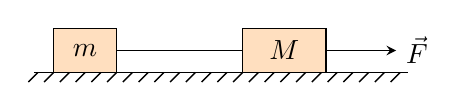
\begin{tikzpicture}[>=stealth,line width=.55pt]\draw[fill=orange!25](0,0)rectangle(.8,.56)node[pos=.5]{$m$};\draw[fill=orange!25](2.4,0)rectangle(3.46,.56)node[pos=.5]{$M$};\draw(.8,.28)--(2.4,.28);\draw[->](3.46,.28)--(4.35,.28)node[right]{$\vec F$};\draw(-.25,0)--(4.5,0);\foreach \x in {-.2,0,...,4.4}{\draw(\x,0)--++(-.12,-.12);}\end{tikzpicture}\end{center}По гладкому горизонтальному столу двигаются два бруска, связанные нерастяжимой и невесомой нитью, которая натянута с силой T  =  $3$ Н. В движение их приводит горизонтально направленная сила F  =  $9$ Н, приложенная к одному из брусков (см. рис.). Чему равна масса M бруска, к которому приложена сила, если масса второго бруска m  =  $0{,}1\,\text{кг}$?
}{
\smallskip\noindent\textbf{Решение}\par
\begin{center}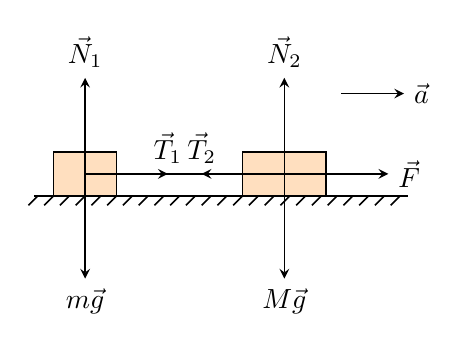
\begin{tikzpicture}[>=stealth,line width=.55pt]\draw[fill=orange!25](0,0)rectangle(.8,.56) (2.4,0)rectangle(3.46,.56);\draw(.8,.28)--(2.4,.28) (-.25,0)--(4.5,0);\foreach \x in {-.2,0,...,4.4}{\draw(\x,0)--++(-.12,-.12);}\draw[->](.4,.28)--(.4,1.5)node[above]{$\vec N_1$};\draw[->](.4,.28)--(.4,-1.05)node[below]{$m\vec g$};\draw[->](.4,.28)--(1.45,.28)node[above]{$\vec T_1$};\draw[->](2.93,.28)--(2.93,1.5)node[above]{$\vec N_2$};\draw[->](2.93,.28)--(2.93,-1.05)node[below]{$M\vec g$};\draw[->](2.93,.28)--(1.88,.28)node[above]{$\vec T_2$};\draw[->](2.93,.28)--(4.25,.28)node[right]{$\vec F$};\draw[->](3.65,1.3)--(4.45,1.3)node[right]{$\vec a$};\end{tikzpicture}\end{center}Изобразим силы, действующие на каждый из брусков. Нить невесома, поэтому силы натяжения $T_1 = T_2 = T.$ Нить нерастяжима, поэтому оба бруска движутся с одинаковым ускорением. Запишем второй закон Ньютона для каждого бруска:

$\overrightarrow{N}_1 + \overrightarrow{T}_1 + m \vec{g} = m \vec{a},$
$\overrightarrow{F} + \overrightarrow{N}_2 + \overrightarrow{T}_2 + M \vec{g} = M \vec{a}.$

 В проекции на горизонтальную ось, сонаправленную с вектором ускорения, получаем:

$F - T = Ma,$
$T = ma.$

 Из этих уравнений находим массу большого бруска:

\[M = \frac{m ( F - T )}{T} = \frac{0{,}1 \cdot ( 9 - 3 )}{3} = 0{,}2 \,\text{кг}.\]

Ответ: $0{,}2\,\text{кг}$.
}

% Source 3024: https://phys-ege.sdamgia.ru/problem?id=3024
\BankTask{3024}{
Горизонтальный проводящий стержень прямоугольного сечения поступательно движется с ускорением вверх по гладкой наклонной плоскости в вертикальном однородном магнитном поле (см. рис.).
\begin{center}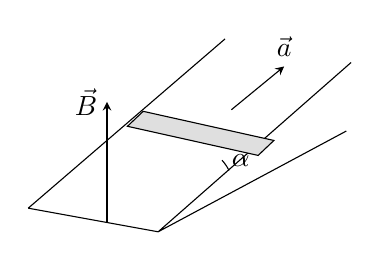
\begin{tikzpicture}[>=stealth]

\draw (0,.3)--(1.65,0)--(4.1,2.15) (0,.3)--(2.5,2.45) (1.65,0)--(4.04,1.28);
\draw (2.55,.78) arc(27:42:.6) node[right]{$\alpha$};
\draw[fill=gray!25] (1.26,1.34)--(2.92,.97)--(3.12,1.16)--(1.46,1.53)--cycle;
\draw[->] (2.58,1.55)--(3.25,2.1) node[above]{$\vec a$};\draw[->] (1,.13)--(1,1.65) node[left]{$\vec B$};
\end{tikzpicture}\end{center}

По стержню протекает ток I. Угол наклона плоскости $\alpha = 30 ^\circ.$ Отношение массы стержня к его длине $\frac{m}{L} =0{,}1\,\text{кг/м}.$ Модуль индукции магнитного поля $B = 0{,}2\,\text{Тл}.$ Ускорение стержня $a = 1{,}9\,\text{м/с} ^2 .$ Чему равна сила тока в стержне?
}{
\smallskip\noindent\textbf{Решение}\par
\begin{center}\begin{tikzpicture}[>=stealth]

\draw (0,0)--(3.2,0);\draw[->] (0,0)--(3.2,1.85) node[right]{$x$};\draw (.65,0)arc(0:30:.65)node[midway,right]{$\alpha$};
\draw[fill=gray!20,rotate=30] (1.1,0)rectangle(2,.43);
\coordinate (M) at (1.34,.79);\draw[->] (M)--(2.68,.79)node[right]{$\vec F_{\!\text{А}}$};
\draw[->] (M)--(.71,1.88) node[above]{$\vec N$};\draw[->] (M)--(1.34,-.55) node[below]{$m\vec g$};
\end{tikzpicture}\end{center}
$1$.  На рисунке показаны силы, действующие на стержень с током:
—  сила тяжести $m\vec{g},$ направленная вертикально вниз; 
—  сила реакции опоры $\vec{N},$ направленная перпендикулярно к наклонной плоскости;
—  сила Ампера $\vec F_{\,\text{А}},$ направленная горизонтально вправо, что вытекает из условия задачи.
$2$.  Модуль силы Ампера $F_{\,\text{А}}=IBL \sin \beta ,$ где  угол между направлением тока и вектором магнитной индукции $\sin \beta =1.$
$3$.  Систему отсчета, связанную с наклонной плоскостью, считаем инерциальной. Для решения задачи достаточно записать второй закон Ньютона $\vec{N} + \vec F_A + m \vec{g}=m \vec{a} .$ 
В проекциях на ось х (см. рис.):

\[ma= - mg \sin \alpha + IBL \cos \alpha .\]

Отсюда находим $I= \frac{m ( a + g \sin \alpha )}{LB \cos \alpha} = \frac{0{,}1 \cdot ( 1{,}9 + 10 \cdot \sin 30 ^\circ )}{0{,}2 \cdot \cos 30 ^\circ} \approx 4\,\text{А}.$

Ответ: $I\approx 4\,\text{А}.$
}

% Source 43028: https://phys-ege.sdamgia.ru/problem?id=43028
\BankTask{43028}{
В вакууме в однородное горизонтальное электрическое поле с напряженностью E  =  $1000$ кВ/м помещают неподвижную капельку массой m  =  $0{,}4\,\text{г}$ и зарядом q  =  $3\,\text{нКл}$. Определите скорость капельки через t  =  $0{,}2\,\text{с}$. Сделайте рисунок, на котором укажите силы, действующие на капельку.
}{
\smallskip\noindent\textbf{Решение}\par
\begin{center}\begin{tikzpicture}[>=stealth]

\draw[->](-.65,1.05)--(2.55,1.05)node[midway,above]{$\vec E$};
\fill (0,.38) circle(.055);\draw[->](0,.38)--(1.25,.38) node[right]{$\vec F_{\!\text{э}}$};\draw[->](0,.38)--(0,-.65)node[below]{$m\vec g$};
\end{tikzpicture}\end{center}
На капельку действуют сила тяжести $m \vec{g}$ и сила действия электрического поля, направленная по линиям напряженности и равная $F_{\,\text{э}}=Eq.$
Равнодействующая этих сил постоянна и по второму закону Ньютона равна 

\[m \vec{g} + \vec F_{\,\text{э}}=m \vec{a} .\]

По горизонтальной оси: проекция ускорения капельки

\[a_x= \frac{Eq}{m} ,\]

тогда проекция скорости на горизонтальную ось при равноускоренном движении без начальной скорости

\[v _x= a_xt= \frac{Eqt}{m} .\]

По вертикали под действием силы тяжести $a_y=g,$ поэтому вертикальная проекция скорости капельки равна 

\[v _y=gt.\]

Тогда скорость капли через промежуток времени t равна

\[v = \sqrt{v _x ^2 + v _y ^2} =t \sqrt{( \frac{Eq}{m} ) ^2 + g ^2} =0{,}2 \cdot \sqrt{( \frac{3 \cdot 10^{-9} \cdot 10^{6}}{4 \cdot 10 ^{ - 4 }} ) ^2 + 100} =2{,}5 \,\text{м/с} .\]

Ответ: $2{,}5\,\text{м/с}$.
}

% Source 35184: https://phys-ege.sdamgia.ru/problem?id=35184
\BankTask{35184}{
\begin{center}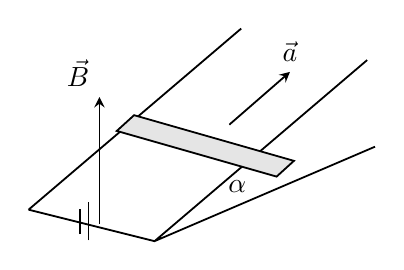
\begin{tikzpicture}[>=stealth,line width=.65pt]\draw (0,0)--(1.6,-.4)--(4.3,1.9) (0,0)--(2.7,2.3) (1.6,-.4)--(4.4,.8);\draw[fill=gray!20] (1.12,1)--(3.15,.42)--(3.37,.62)--(1.34,1.2)--cycle;\draw[->] (.9,-.18)--(.9,1.43) node[above left]{$\vec B$};\draw[->] (2.55,1.08)--(3.32,1.75) node[above]{$\vec a$};\draw (.65,-.31)--(.65,.01) (.76,-.39)--(.76,.1);\node at (2.65,.3){$\alpha$};\end{tikzpicture}\end{center}

 Горизонтальный проводящий стержень прямоугольного сечения поступательно движется с ускорением вверх по гладкой наклонной плоскости в вертикальном однородном магнитном поле (см. рис.). По стержню протекает ток $I=4\,\text{А}.$ Угол наклона плоскости $\alpha =30 ^\circ.$ Отношение массы стержня к его длине $\frac{m}{L} =0{,}1\,\text{кг/м}.$ Модуль индукции магнитного поля $B=0{,}2\,\text{Тл}.$ Чему равно ускорение стержня?
}{
\smallskip\noindent\textbf{Решение}\par
\begin{center}\begin{tikzpicture}[>=stealth,line width=.65pt]\draw (0,0)--(4,0) (0,0)--(3.4,1.95);\draw (.48,0) arc (0:30:.48) node[right]{$\alpha$};\draw[fill=gray!20,rotate=30] (1.45,0) rectangle (2.45,.55);\coordinate (o) at (1.55,1.2);\draw[->](o)--++(2.25,1.3)node[above]{$x$};\draw[->](o)--++(-1.1,1.9)node[left]{$y$};\draw[->,thick](o)--++(-.5,.87)node[below left]{$\vec N$};\draw[->,thick](o)--++(1.5,0)node[right]{$\vec F_{\text{А}}$};\draw[->,thick](o)--++(0,-1)node[below]{$m\vec g$};\draw (2.12,1.2) arc (0:30:.57);\node at (2.28,1.38){$\alpha$};\draw (1.55,.58) arc (-90:-60:.62);\node at (1.89,.5){$\alpha$};\end{tikzpicture}\end{center}

На стержень действуют сила тяжести mg, сила Ампера $F_{A}$ и сила реакции опоры N. Изобразим эти силы на рисунке.
По второму закону Ньютона $m\vec{g} + \vec{N} + \vec F_A=m\vec{a}.$
В проекции на выбранную ось Oх:

\[F_A \cos \alpha - mg \sin \alpha =ma.\]

Сила Ампера находится по формуле $F_A = BIl \sin \beta ,$ где $\beta$  =  $90$\ensuremath{{}^{\circ}}  — угол между направлением тока и вектором магнитной индукции.
Тогда получаем:

\[ma + mg \sin \alpha = BIl \cos \alpha .\]

Отсюда ускорение стержня равно:

\[a= \frac{BIl \cos \alpha}{m} - g \sin \alpha = \frac{0{,}2 \cdot 4 \cdot \cos 30 ^\circ}{0{,}1} - 10 \cdot 0{,}5\approx 1{,}9 \,\text{м/с} ^2 .\]

Ответ: $1{,}9\,\text{м/с}^{2}$.
}

% Source 25774: https://phys-ege.sdamgia.ru/problem?id=25774
\BankTask{25774}{
Имеется недеформированная пружина длиной $L$  =  $30\,\text{см}$ и жесткостью $k$  =  $30\,\text{Н/м}$, груз массой $m$  =  $1\,\text{кг}$, а также вращающийся с частотой $\nu = 0{,}5\,\text{Гц}$ массивный диск. На каком минимальном расстоянии от центра диска можно положить на него груз, прикрепив его пружиной к центру диска, чтобы груз оставался неподвижным относительно диска? Коэффициент трения между грузом и диском $\mu=0{,}5.$ Размерами груза пренебречь. Сделайте схематический рисунок с указанием сил, действующих на груз.
Какие законы Вы использовали для описания движения бруска? Обоснуйте их применимость к данному случаю.
}{
\smallskip\noindent\textbf{Решение}\par
Обоснование. 
$1$.  Рассмотрим задачу в инерциальной системе отсчета, связанной с Землей. Будем считать эту систему отсчета инерциальной (ИСО). Тело описываем моделью материальной точки, так как его размеры малы по сравнению с диском. 
$2$.  При вращении диска на тело действуют потенциальная сила тяжести, сила реакции опоры, перпендикулярная опоре, потенциальная сила упругости, возникающая в упруго деформированной пружине и сила трения покоя. Работа силы тяжести и силы реакции опоры равны нулю. 
$3$.  Поскольку тело описывается моделью материальной точки, в ИСО применим второй закон Ньютона. Равнодействующая сила направлена к центру, следовательно, тело движется с центростремительным ускорением. Для материальной точки применимы законы равномерного движения по окружности.
$4$.  При малых деформациях их можно считать упругими, поэтому для пружины верен закон Гука.
$5$.  Брусок покоится относительно диска, имеющего шероховатую поверхность. Поэтому на него действует максимальная сила трения покоя, равная силе трения скольжения $F_{\,\text{тр}}=\mu N.$

Перейдем к решению. \begin{center}\begin{tikzpicture}[task graph,>=stealth]\draw(.1,0)--(5,0)--(5,-.4)--(.1,-.4);\draw[dashed](.1,0)--(-.85,0)--(-.85,-.4)--(.1,-.4);\draw(-.4,-.4)--(.1,-.4)--(.1,1.8);\draw[very thick](.1,-.4)--(.1,1.8);\draw[fill=gray!15](3,.05)rectangle(4.2,.85);\draw(.1,.45)--(.3,.45);\draw plot[domain=0:1,samples=100]({.3+2.7*\x},{.45+.15*sin(2880*\x)});\node[below right]at(5.2,-1.1){$O$};\draw[->](5.2,-1.1)--(5.2,2.1)node[above]{$y$};\draw[->](5.2,-1.1)--(1.2,-1.1)node[left]{$x$};\draw[->](.1,1.8)..controls(-.5,2.3)and(.6,2.3)..(.1,1.8)node[above left]{$\nu$};\draw[->,thick](3.6,.45)--(3.6,2.3)node[above]{$\vec N$};\draw[->,thick](3.6,.45)--(3.6,-.9)node[right]{$m\vec g$};\draw[->,thick](3.6,.45)--(5,.45)node[right]{$\vec F_{\text{упр}}$};\draw[->,thick](3.6,.45)--(1.9,.45)node[above left]{$\vec F_{\text{тр}}$};\draw[->,thick](2.6,2.3)--(1.4,2.3)node[above left]{$\vec a_{\text{ц}}$};\end{tikzpicture}\end{center} 
$1$.  На груз действуют четыре силы: сила тяжести $m\vec g,$ нормальная составляющая силы реакции опоры $\overrightarrow{N},$ сила упругости $\overrightarrow{F}_{\,\text{упр}}$ и сила трения $\overrightarrow{F}_{\,\text{тр}}.$
Выясним, в каком состоянии будет находиться пружина. Если грузик находится на расстоянии $L$ от центра, то равнодействующая сила равна $ma=4 \pi ^2 \nu ^2 Lm=3$$H$. Максимальная сила трения равна $F_{\,\text{т}} =\mu mg =5$$H$. Значит, пружина должна быть сжата, сила упругости направлена вправо (см. рис.), а сила трения  — влево. Поскольку пружина максимально сжата, а груз при этом находится в покое относительно диска, сила трения покоя принимает максимальное значение: $F_{\,\text{тр}}=\mu N.$
$2$.  Второй закон Ньютона в проекциях на оси инерциальной системы отсчета XOY имеет вид: $OX: ma_{\,\text{ц}}=F_{\,\text{тр}} - F_{\,\text{упр}};$ $OY: 0=N - mg.$ Сила упругости определяется законом Гука: $F_{\,\text{упр}}=k\Delta x.$ Центростремительное ускорение груза выражается формулой $a_{\,\text{ц}}= \frac{V ^2}{R_{\min}} =4 \pi ^2 \nu ^2 R_{\min}.$
$3$.  Из формул, приведенных выше, получаем: $4 \pi ^2 \nu ^2 R_{\min}m=\mu mg - k\Delta x,$ где $R_{\min}=L - \Delta x.$ Окончательно получим:

\[R_{\min}= \frac{kL - \mu mg}{k - 4 \pi ^2 \nu ^2 m} = \frac{30 \cdot 0{,}3 - 0{,}5 \cdot 1 \cdot 10}{30 - 4 \cdot 3{,}14 ^2 \cdot 0{,}5 ^2 \cdot 1} \approx 0{,}2 \,\text{м}.\]

Ответ: $R_{\min}\approx 0{,}2 \,\text{м}.$
}

% Source 38208: https://phys-ege.sdamgia.ru/problem?id=38208
\BankTask{38208}{
\begin{center}\begin{tikzpicture}[task graph,>=stealth]
\draw(0,0)--(5,0)--(5,2.887)--cycle;\draw(-.3,0)--(6.4,0);
\begin{scope}[shift={(2.8,1.6166)},rotate=30]\draw(0,0)rectangle(1.1,.5);\node at(.55,.8){$m$};\end{scope}
\node at(4.4,1.2){$M$};\draw[->](5,1.45)--(6.4,1.45)node[above]{$\vec F$};
\draw(.85,0)arc(0:30:.85);\node at(1.1,.27){$\alpha$};
\end{tikzpicture}\end{center}Под действием постоянной горизонтальной силы $\vec F$ клин массой $M = 1 \,\text{кг}$  движется по гладкой горизонтальной поверхности стола. По шероховатой поверхности клина, составляющей угол $\alpha = 30 ^{ \circ }$ с горизонтом, равномерно (относительно клина) скользит вниз брусок массой $m = 0{,}2 \,\text{кг}.$ Коэффициент трения между бруском и клином $\mu = 0{,}6.$ Найдите модуль ускорения клина. Сопротивлением воздуха пренебречь. Сделайте рисунок с указанием сил, действующих на брусок. Обоснуйте применимость законов, используемых для решения задачи.
}{
\smallskip\noindent\textbf{Решение}\par
\begin{center}\begin{tikzpicture}[task graph,>=stealth]\draw[->](-.5,-1.4)--(6,-1.4)node[right]{$x$};\draw[->](-.5,-1.4)--(-.5,3.7)node[above]{$y$};\draw(0,0)--(4.5,0)--(4.5,2.598)--cycle;\begin{scope}[shift={(2.5,1.65)},rotate=30]\draw[fill=gray!15](-.4,-.18)rectangle(.4,.18);\end{scope}\draw(.7,0)arc(0:30:.7)node[midway,right]{$\alpha$};\node at(3.9,1.3){$M$};\node[above]at(2.5,2){$m$};\draw[->,thick](2.5,1.65)--(1.85,2.776)node[above left]{$\vec N_1$};\draw[->,thick](2.5,1.65)--(3.8,2.4)node[above]{$\vec F_{\text{тр}1}$};\draw[->,thick](2.5,1.65)--(2.5,.3)node[right]{$m\vec g$};\draw[->,thick](2.1,0)--(2.1,1.1)node[left]{$\vec N_2$};\draw[->,thick](2.1,0)--(2.1,-1.1)node[below left]{$M\vec g$};\draw[->,thick](2.1,0)--(1,-.635)node[below left]{$\vec F_{\text{тр}2}$};\draw[->,thick](2.1,0)--(2.7,-1.039)node[right]{$\vec P$};\draw[->,thick](4.5,1.2)--(5.8,1.2)node[right]{$\vec F$};\draw[->,thick](5,2.8)--(6,2.8)node[above]{$\vec a$};\end{tikzpicture}\end{center}Обоснование:
Систему отсчета, связанную с Землей, будем считать инерциальной. Движение бруска поступательное. Следовательно, его можно считать материальной точкой. 
При движении бруска по плоскости клина на него действуют силы тяжести $mg$, трения скольжения $F_{\,\text{тр}1}$  и реакции опоры $N_1.$ На клин действуют сила тяжести Mg, сила трения между бруском и клином $F_{\,\text{тр}2},$ сила реакции опоры $N_2,$ вес бруска P и приложенная горизонтальная сила F. Движение клина по горизонтальной поверхности поступательное. Следовательно, его можно описывать моделью материальной точки.
Так как брусок относительно клина движется равномерно, то клин и брусок относительно Земли движутся с одинаковым ускорением a. В ИСО для обоих тел выполняется второй закон Ньютона.
Силы трения между бруском и клином – парные, по третьему закону Ньютона эти силы равны по модулю в ИСО. Вес бруска по третьему закону Ньютона равен силе реакции опоры $N_{1}$.
Перейдем к решению.
Запишем второй закон Ньютона для бруска:

\[\vec F_{\,\text{тр}} + m\vec g + \vec N_1=m\vec a.\]

Выберем оси: $Ox$ направим горизонтально вправо, $Oy$ направим вертикально вверх. В проекциях на координатные оси:

$Ox$: $- N_1 \sin \alpha + F_{\,\text{тр}} \cos \alpha =ma;$
$Oy$: $N_1 \cos \alpha + F_{\,\text{тр}} \sin \alpha - mg=0.$

Сила трения между бруском и поверхностью клина $F_{\,\text{тр}}=\mu N_1.$
Решая данную систему, находим ускорение бруска: $a= \frac{g ( \mu - \tan \alpha )}{1 + \mu \tan \alpha} .$
Подставляя числовые значения, находим ускорение бруска (равное ускорению клина):

\[a= \frac{10 \cdot ( 0{,}6 - \tan 30 ^\circ )}{1 + 0{,}6 \cdot \tan 30 ^\circ} \approx 0{,}17 \,\text{м/с} ^2 .\]

Ответ: $0{,}17\,\text{м/с}^{2}$.
}

% Source 41585: https://phys-ege.sdamgia.ru/problem?id=41585
\BankTask{41585}{
\begin{center}\begin{tikzpicture}[task graph,>=stealth]
\draw(0,0)--(6.4,0);\foreach \x in {.2,.4,...,6.4}{\draw(\x,0)--++(-.12,-.12);}
\draw(1.2,0)rectangle(2.7,2.8);\node at(1.95,1.8){$M$};
\draw[->](1.2,1.3)--(.1,1.3)node[above]{$\vec F$};
\draw(2.7,1.3)--(3.1,1.3);\draw(3.1,1.3)circle(.4);\fill(3.1,1.3)circle(1pt);
\draw(6.2,1.7)--(3.1,1.7)arc(90:270:.4)--(4.8,.9);
\draw(4.8,0)rectangle(6,1.2);\node at(5.4,.6){$m$};
\draw(6.2,.9)--(6.2,2.8);\foreach \y in {1,1.2,...,2.8}{\draw(6.2,\y)--++(.12,.12);}
\end{tikzpicture}\end{center}Брусок массой $M$  =  $2\,\text{кг}$ соединен с лёгким блоком (см. рисунок), через него переброшена лёгкая нерастяжимая нить, один конец которой привязан к стене, а к другому прикреплено тело массой $m$  =  $0{,}75\,\text{кг}$. На брусок действует сила F  =  $10$ $H$. Определите ускорение бруска. Свободные куски нити горизонтальны и лежат в одной вертикальной плоскости, тела двигаются вдоль одной прямой. Массой блока и нити, а также трением пренебречь.
Обоснуйте применимость законов, используемых для решения задачи.
}{
\smallskip\noindent\textbf{Решение}\par
Обоснование.
Рассмотрим движение тел в системе отсчета, связанной с Землей, которую в данных условиях можно считать инерциальной системой отсчета.
Брусок и тело движутся поступательно, поэтому их можно описывать моделью материальной точки.
Нить невесома, блок идеален (отсутствует трение, массой пренебрегаем), поэтому силы натяжения нити равны $T_1=T_2=T.$
В инерциальной системе отсчета для материальных точек можно применять законы Ньютона.
Так как нить нерастяжима, перемещение тела в $2$ раза больше перемещения бруска, то ускорения бруска и тела кинематически связаны соотношением $a_1=2a_2.$
Перейдем к решению. 
\begin{center}\begin{tikzpicture}[task graph,>=stealth]\draw(-1,0)--(6.2,0);\draw[fill=gray!10](0,0)rectangle(1.5,2.8);\node at(.6,.7){$M$};\draw(1.5,1.35)--(2.1,1.35);\draw(2.1,1.35)circle(.4);\draw(2.1,1.75)--(5.8,1.75);\draw(2.1,.95)--(4.3,.95);\draw[fill=gray!15](4.3,0)rectangle(5.2,.95);\node at(4.75,.5){$m$};\draw(5.8,.65)--(5.8,2.5);\foreach \yy in {.75,.95,...,2.45}{\draw(5.8,\yy)--++(.17,-.17);}\foreach \xx in {-.8,-.3,...,5.7}{\draw(\xx,0)--++(.3,-.13);}\draw[->,thick](0,1.35)--(-1.1,1.35)node[above left]{$\vec F$};\draw[->,thick](2.1,1.35)--(.9,1.35)node[above left]{$\vec T_3$};\draw[->,thick](2.1,1.75)--(3.4,1.75)node[above]{$\vec T_2$};\draw[->,thick](2.1,.95)--(3.4,.95)node[below]{$\vec T_2$};\draw[->,thick](4.3,.95)--(3.5,.95)node[above]{$\vec T_1$};\draw[->,thick](1.5,.25)--(2.8,.25)node[below]{$\vec T_4$};\draw[->,thick](.8,3.2)--(-.3,3.2)node[above]{$\vec a_2$};\draw[->,thick](5.1,-.45)--(4.2,-.45)node[below]{$\vec a_1$};\end{tikzpicture}\end{center}
Для блока по третьему закону Ньютона силы взаимодействия блока и бруска $T_3=T_4.$ Так как блок невесомый, то $T_4=2T_2=2T.$
Применим второй закон Ньютона на бруска и тела:

$\vec F + \vec T_4=M\vec a_2;$
$\vec T_1=m\vec a_1.$

В проекции на горизонтальную ось имеем:

$F - 2T=Ma_2;$
$T=2ma_2.$

При объединении получаем:

\[F - 4ma_2=Ma_2,\]

откуда находим ускорение бруска:

\[a_2= \frac{F}{M + 4m} = \frac{10}{2 + 4 \cdot 0{,}75} =2 \,\text{м/с} ^2 .\]

Ответ: $2\,\text{м/с}^{2}$.
}

% Source 25727: https://phys-ege.sdamgia.ru/problem?id=25727
\BankTask{25727}{
На горизонтальном столе лежит деревянный брусок. Коэффициент трения между поверхностью стола и бруском $\mu$ = $0{,}1$. Если приложить к бруску силу, направленную вверх под углом $\alpha$ = $45$° к горизонту, то брусок будет двигаться по столу равномерно. С каким ускорением будет двигаться этот брусок по столу, если приложить к нему такую же по модулю силу, направленную под углом $\beta$ = $30^{\circ}$ к горизонту?
Какие законы Вы используете для описания движения бруска? Обоснуйте их применение к данному случаю.
}{
\smallskip\noindent\textbf{Решение}\par
Обоснование. 
$1$.  Рассмотрим задачу в системе отсчета, связанной с Землей. Будем считать эту систему отсчета инерциальной (ИСО).
$2$.  Брусок движется поступательно, поэтому описываем его моделью материальной точки. В ИСО движение материальной точки описываем вторым законом Ньютона.
$3$.  Так как брусок движется поступательно по шероховатой поверхности, то действует сила трения скольжения $F_{\,\text{тр}}=\mu N.$

Перейдем к решению. \begin{center}\begin{tikzpicture}[task graph,>=stealth]\draw(-1.8,0)--(2.2,0);\draw[fill=gray!15](-.5,0)rectangle(.5,.5);\coordinate(C)at(0,.25);\draw[dashed](0,.25)--(1.8,.25);\draw[dashed](0,1.3813708498984762)--(1.1313708498984762,1.3813708498984762)--(1.1313708498984762,.25);\draw(C)++(0:.6)arc(0:45:.6)node[midway,right]{$\alpha$};\draw(1.13137,1.38137)++(180:.4)arc(180:225:.4)node[midway,left]{$\alpha$};\draw[->,thick](C)--(1.1313708498984762,1.3813708498984762)node[above right]{$\vec F_{\text{т}}$};\draw[->,thick](C)--(0,1.9)node[above left]{$\vec N$};\draw[->,thick](C)--(0,-1)node[below]{$m\vec g$};\draw[->,thick](C)--(-1.5,.25)node[above left]{$\vec F_{\text{тр}}$};\end{tikzpicture}\end{center}
$1$.  Ускорение равно нулю, так как движение равномерное.

$\vec N + m\vec g + \vec F_{\,\text{тр}} + \vec F_{\,\text{т}} = m\vec a = 0.$

OX: $F_{\,\text{т}} \cos \alpha - \mu N = 0 \Longleftrightarrow F_{\,\text{т}} \cos \alpha = \mu N. ( 1 )$
OY: $N + F_{\,\text{т}} \sin \alpha = mg \Longleftrightarrow N= mg - F_{\,\text{т}} \sin \alpha . ( 2 )$

Из первого и второго уравнения получаем:

\[F_{\,\text{т}} \cos \alpha =\mu mg - \mu F_{\,\text{т}} \sin \alpha \Rightarrow F_{\,\text{т}}= \frac{\mu mg}{\cos \alpha + \mu \sin \alpha} . ( 3 )\]

\begin{center}\begin{tikzpicture}[task graph,>=stealth]\draw(-1.8,0)--(2.2,0);\draw[fill=gray!15](-.5,0)rectangle(.5,.5);\coordinate(C)at(0,.25);\draw[dashed](0,.25)--(1.8,.25);\draw[dashed](0,1.0499999999999998)--(1.385640646055102,1.0499999999999998)--(1.385640646055102,.25);\draw(C)++(0:.6)arc(0:30:.6);\draw(1.38564,1.05000)++(180:.4)arc(180:210:.4)node[midway,left]{$\beta$};\draw[->,thick](C)--(1.385640646055102,1.0499999999999998)node[above right]{$\vec F_{\text{т}}$};\draw[->,thick](C)--(0,1.9)node[above left]{$\vec N$};\draw[->,thick](C)--(0,-1)node[below]{$m\vec g$};\draw[->,thick](C)--(-1.5,.25)node[above left]{$\vec F_{\text{тр}}$};\end{tikzpicture}\end{center}$2$.  Ускорение не равно нулю, так как движение с ускорением.

$\vec F_{\,\text{т}} + \vec N_1 + \vec F_{\,\text{тр}1} + m\vec g = m\vec a$
OX: $F_{\,\text{т}} \cos \beta - \mu N_1 = ma \Longleftrightarrow a= \frac{F_{\,\text{т}} \cos \beta - \mu N_1}{m} . ( 4 )$
OY: $N_1 + F_{\,\text{т}} \sin \beta = mg \Longleftrightarrow N_1 = mg - F_{\,\text{т}} \sin \beta . ( 5 )$

Из четвертого и пятого уравнения получаем:

\[a= \frac{F_{\,\text{т}} \cos \beta - \mu mg + F_{\,\text{т}}\mu \sin \beta}{m} = \frac{F_{\,\text{т}} ( \cos \beta + \mu \sin \beta )}{m} - \mu g. ( 6 )\]

Из третьего и шестого уравнения получаем:

\[a= \frac{\mu mg ( \cos \beta + \mu \sin \beta )}{( \cos \alpha + \mu \sin \alpha ) m} - \mu g = \mu g ( \frac{\cos \beta + \mu \sin \beta}{\cos \alpha + \mu \sin \alpha} - 1 )\]

  — уравнение в общем виде.

\[a=0{,}1 \cdot 10 \cdot ( \frac{\cos 30 ^\circ + 0{,}1 \cdot \sin 30 ^\circ}{\cos 45 ^\circ + 0{,}1 \cdot \sin 45 ^\circ} - 1 ) \approx 0{,}18\,\text{м/с} ^2 .\]

Ответ: $0{,}18\,\text{м/с}^{2}$.
}

% Source 43833: https://phys-ege.sdamgia.ru/problem?id=43833
\BankTask{43833}{
На горизонтальном неподвижном столе лежит доска массой $M=0{,}8\,\text{кг}$. На доске находится маленький брусок массой $m=200\,\text{г}$. Брусок и доска связаны невесомой нерастяжимой нитью, перекинутой через невесомый блок, который закреплён на стене (отрезки нити, не лежащие на блоке, горизонтальны). Коэффициент трения между бруском и доской $\mu_1=0{,}5$, между столом и доской $\mu_2=0{,}3$. Доску тянут вправо горизонтальной силой $\vec F$. Чему равен модуль силы $\vec F$, если модуль ускорения бруска относительно стола $a=1\,\text{м/с}^2$? Трением в оси блока пренебречь. Сделайте рисунок с указанием сил, действующих на тела. Обоснуйте применимость законов, используемых для решения задачи.
\begin{center}
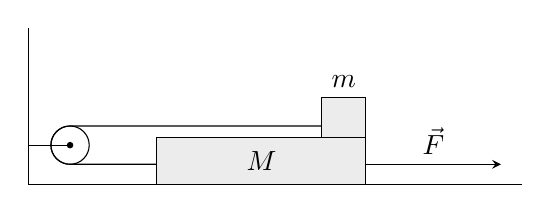
\begin{tikzpicture}[x=.64cm,y=.64cm,>=stealth]
\draw (0,3.1)--(0,0)--(9.8,0);
\draw (0,.78)--(.83,.78);
\draw (.83,.78) circle (.38);
\fill (.83,.78) circle (.065);
\draw (5.82,1.16)--(.83,1.16) arc[start angle=90,end angle=270,radius=.38]--(2.55,.40);
\draw[fill=gray!15] (2.55,0) rectangle (6.7,.94);
\draw[fill=gray!15] (5.82,.94) rectangle (6.7,1.72);
\node at (4.63,.47) {$M$};
\node[above] at (6.26,1.72) {$m$};
\draw[->] (6.7,.40)--(9.38,.40) node[midway,above] {$\vec F$};
\end{tikzpicture}
\end{center}
}{
\smallskip\noindent\textbf{Решение}\par
\textbf{Обоснование}

1. Задачу будем решать в инерциальной системе отсчёта, связанной с поверхностью стола.

2. Тела движутся поступательно, поэтому будем их описывать моделью материальной точки. Следовательно, можно использовать второй закон Ньютона, сформулированный для материальных точек. Силы, действующие на тела, постоянны, поэтому движение бруска и доски равноускоренно.

3. Так как нить нерастяжима, ускорения бруска и доски относительно стола равны по модулю и противоположны по направлению: $|\vec a_1|=|\vec a_2|=a$, $\vec a_1=-\vec a_2$. \hfill(1)

4. Так как блок и нити невесомы и трением в оси блока можно пренебречь, то силы натяжения нити, действующие на доску и брусок, одинаковы: $|\vec T_1|=|\vec T_2|=T$. \hfill(2)

5. Силы трения, действующие на брусок и доску, равны друг другу и противоположны по направлению по третьему закону Ньютона: $\vec F_{\text{тр}1}=-\vec F_{\text{тр}2}$. \hfill(3)

6. Модули сил нормальной реакции доски $\vec N_1$ и давления бруска на доску $\vec P$ также равны друг другу по третьему закону Ньютона: $N_1=P$. \hfill(4)

\textbf{Решение}

1. На рисунке показаны силы, действующие на брусок и на доску. Запишем второй закон Ньютона в проекциях на оси $Ox$ и $Oy$ выбранной системы координат. С учётом (1)–(3) получим:
\[Ma=F-F_{\text{тр}1}-F_{\text{тр}3}-T,\qquad -ma=F_{\text{тр}1}-T,\]
\[N_1=mg,\qquad N_2=Mg+P.\]

\begin{center}
\begin{tikzpicture}[x=.67cm,y=.67cm,>=stealth]
\draw[->] (0,0)--(12.05,0) node[below] {$x$};
\draw[->] (0,0)--(0,3.55) node[left] {$y$};
\node[below left] at (0,0) {$0$};
\draw (0,1.04)--(1.08,1.04);
\draw (1.08,1.04) circle (.50);
\fill (1.08,1.04) circle (.085);
\draw (7.7,1.54)--(1.08,1.54) arc[start angle=90,end angle=270,radius=.50]--(3.4,.54);
\draw[fill=gray!15] (3.4,0) rectangle (8.85,1.2);
\draw[fill=gray!15] (7.7,1.2) rectangle (8.85,2.26);
\draw[->] (8.27,1.73)--(8.27,3.23) node[right] {$\vec N_1$};
\draw[->] (8.27,1.73)--(8.27,.81) node[below right] {$m\vec g$};
\draw[->] (8.27,1.73)--(9.87,1.73) node[right] {$\vec F_{\text{тр}1}$};
\draw[->] (7.7,1.54)--(7.05,1.54) node[above] {$\vec T_1$};
\draw[->] (3.4,.54)--(2.27,.54) node[above] {$\vec T_2$};
\draw[->] (6.1,.64)--(6.1,3.02) node[left] {$\vec N_2$};
\draw[->] (6.1,.64)--(6.1,-1.38) node[right] {$M\vec g$};
\draw[->] (7.48,1.08)--(7.48,.16) node[midway,left] {$\vec P$};
\draw[->] (5.96,.92)--(4.78,.92);
\draw (4.72,1.01)--(3.92,1.60) node[above] {$\vec F_{\text{тр}2}$};
\draw[->] (5.96,.40)--(4.78,.40);
\draw (4.72,.28)--(4.15,-.34) node[below] {$\vec F_{\text{тр}3}$};
\draw[->] (8.85,.54)--(11.13,.54) node[above] {$\vec F$};
\end{tikzpicture}
\end{center}
2. Вычтя второе уравнение из первого, найдём силу, действующую на доску:
\[F=(M+m)a+2F_{\text{тр}1}+F_{\text{тр}3}.\]
3. Далее $F_{\text{тр}1}=\mu_1N_1=\mu_1mg$. С учётом (4) получим $F_{\text{тр}3}=\mu_2N_2=\mu_2(M+m)g$. В итоге:
\[\begin{aligned}F&=(M+m)(a+\mu_2g)+2\mu_1mg\\&=(0{,}8+0{,}2)(1+0{,}3\cdot10)+2\cdot0{,}5\cdot0{,}2\cdot10=6\,\text{Н}.\end{aligned}\]
Ответ: $F=6\,\text{Н}$.
}

% Source 38623: https://phys-ege.sdamgia.ru/problem?id=38623
\BankTask{38623}{
В установке, изображённой на рисунке, масса грузика $m$ подобрана так, что первоначально покоящаяся тележка после толчка вправо движется равномерно по поверхности трибометра. С каким ускорением будет двигаться тележка, если её толкнуть влево? Масса грузика $m$ в $9$ раз меньше массы тележки $M$. Блок идеален. Нить невесома и нерастяжима. Силу сопротивления движению тележки считать постоянной и одинаковой в обоих случаях. Обоснуйте применимость законов, используемых для решения задачи.
\begin{center}
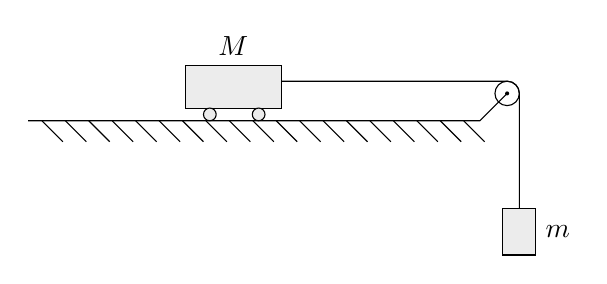
\begin{tikzpicture}[x=.62cm,y=.62cm]
\draw (0,0)--(9.25,0)--(9.81,.56);
\foreach \x in {.28,.76,...,8.96} {\draw (\x,0)--++(.43,-.43);}
\draw (9.81,.56) circle (.25);
\fill (9.81,.56) circle (.042);
\draw (5.18,.81)--(9.81,.81) arc[start angle=90,end angle=0,radius=.25]--(10.06,-1.80);
\draw[fill=gray!15] (3.22,.26) rectangle (5.18,1.13);
\draw[fill=gray!15] (3.72,.13) circle (.13);
\draw[fill=gray!15] (4.72,.13) circle (.13);
\node[above] at (4.2,1.13) {$M$};
\draw[fill=gray!15] (9.72,-1.80) rectangle (10.40,-2.75);
\node[right] at (10.40,-2.275) {$m$};
\end{tikzpicture}
\end{center}
}{
\smallskip\noindent\textbf{Решение}\par
\textbf{Обоснование.}

1. Рассмотрим задачу в системе отсчета, связанной с Землей. Будем считать эту систему отсчета инерциальной (ИСО).

2. Грузик и тележка движутся поступательно, поэтому описываем их моделью материальной точки. В ИСО движение материальной точки описываем вторым законом Ньютона.

3. Нить невесома, блок идеален (масса блока ничтожна, трения нет), поэтому модуль силы натяжения нити в любой ее точке одинаковый.

4. Нить нерастяжима, при прямолинейном поступательном движении модули ускорений грузика и тележки будут одинаковыми.

5. Движение тележки поступательное по шероховатой поверхности, поэтому на нее действует сила трения скольжения.

Перейдем к решению.

В горизонтальном направлении на тележку действуют сила трения и сила натяжения нити. В первом случае силы направлены в разные стороны и компенсируют друг друга, поэтому тележка движется равномерно. Во втором случае они обе направлены против движения, тележка движется равнозамедленно. Запишем для них второй закон Ньютона для тележки и грузика в первом случае:
\[\vec T_1+\vec F_{\text{тр}}=0,\qquad \vec T_1+m\vec g=0.\]
В проекции на оси получаем:
\[T_1-F_{\text{тр}}=0,\qquad T_1-mg=0.\]
Откуда получаем: $F_{\text{тр}}=mg$.

Запишем для них второй закон Ньютона для тележки и грузика во втором случае:
\[\vec T_2+\vec F_{\text{тр}}=M\vec a,\qquad \vec T_2+m\vec g=m\vec a.\]
В проекции на оси получаем:
\[T_2+F_{\text{тр}}=Ma,\qquad mg-T_2=ma.\]
Решая систему уравнений, имеем: $a(M+m)=F_{\text{тр}}+mg=2mg$.

В результате находим ускорение тележки:
\[a=\frac{2mg}{M+m}=\frac{2mg}{m+9m}=\frac g5=\frac{10}{5}=2\,\text{м/с}^2.\]
Ответ: $2\,\text{м/с}^2$.
}

% Source 50800: https://phys-ege.sdamgia.ru/problem?id=50800
\BankTask{50800}{
\begin{center}\begin{tikzpicture}[task graph,>=stealth]\draw(-1.15,3.57)--(1.1,3.57);\foreach \x in {-1.1,-.8,...,1.0}{\draw(\x,3.57)--++(.24,.24);}\draw(0,3.57)--(0,2.18) circle(.75);\draw(-.75,2.18)--(-.75,-.20) (.75,2.18)--(.75,-.83);\draw[fill=gray!15](-1.29,-.96)rectangle(-.21,-.20)node[midway]{\(M\)};\draw[fill=gray!15](.22,-1.59)rectangle(1.28,-.83)node[midway]{\(M\)};\draw[fill=gray!30](.50,-.83)rectangle(1.0,-.38)node[midway,right,xshift=9pt]{\(m\)};\end{tikzpicture}\end{center}Два одинаковых бруска массой M  =  $500\,\text{г}$ связаны между собой невесомой нерастяжимой нитью, перекинутой через невесомый гладкий блок, неподвижно закреплённый на потолке (см. рис.). На один из блоков кладут груз массой m  =  $100\,\text{г}$, и система приходит в движение. С какой силой F груз будет давить на брусок? Сделайте схематический рисунок с указанием сил, действующих на бруски и груз. Обоснуйте применимость законов, используемых для решения задачи.
}{
\smallskip\noindent\textbf{Решение}\par
Обоснование. Cистему отсчета, связанную с Землей, будем считать инерциальной. Так как движение грузов поступательное, то их можно описывать моделью материальной точки. Значит, можно применять законы Ньютона для описания движения грузов. Нить, которая связывает тело массой М и тело массой M + m с перегрузком, является невесомой, а блок  — идеальным (его масса равна нулю, трением в его оси вращения можно пренебречь). Следовательно, на оба тела действует одинаковая по модулю сила натяжения нити. Кроме того, нить нерастяжима. Поэтому оба тела движутся с одинаковым по модулю ускорением.

\begin{center}\begin{tikzpicture}[task graph,>=stealth]\draw(-1.15,3.57)--(1.1,3.57);\foreach \x in {-1.1,-.8,...,1.0}{\draw(\x,3.57)--++(.24,.24);}\draw(0,3.57)--(0,2.18) circle(.75);\draw(-.75,2.18)--(-.75,-.20) (.75,2.18)--(.75,-.83);\draw[fill=gray!15](-.94,-1.07)rectangle(-.56,-.40)(.56,-1.66)rectangle(.94,-.7);\draw[->] (0,2.18)--(0,3.4) node[right]{\(\vec F\)};\draw[->] (0,2.18)--(0,.92) node[right]{\(\vec F\)};\draw[->] (-.75,2.18)--(-.75,.92) node[right]{\(\)};\draw[->] (.75,2.18)--(.75,.92) node[right]{\(\)};\draw[->] (-.75,-.73)--(-.75,.6) node[left]{\(\vec T_1\)};\draw[->] (.75,-1.2)--(.75,.35) node[right]{\(\vec T_2\)};\draw[->] (-.75,-.73)--(-.75,-1.69) node[left]{\(M\vec g\)};\draw[->] (.75,-1.2)--(.75,-2.4) node[right]{\((M+m)\vec g\)};\draw[->] (2.66,3.3)--(2.66,-1.42) node[right]{\(X\)};\end{tikzpicture}\end{center}
Перейдем к решению. Запишем, на основании второго закона Ньютона, уравнения движения для обоих грузов в проекции на вертикальную ось, направленную вниз (см. рис.):

$Ma_1=Mg - T_1,$ $( M + m ) a_2= ( M + m ) g - T_2.$

Здесь через $a_1$ и $a_2$ обозначены проекции ускорений грузов M и $( M + m )$ на вертикальную ось, а через $T_1$ и $T_2$  — проекции сил натяжения нити на ту же ось.
В силу условия задачи из-за нерастяжимости нити $a_1= - a_2= - a,$ а из-за невесомости блока и нити и отсутствия трения$T_1=T_2=T.$ 
Из написанных уравнений получаем: 

\[a= \frac{m}{m + 2M} g.\]

Рассмотрим движение только перегрузка. Он давит на груз силой, которая по третьему закону Ньютона равна $F=N.$ Запишем второй закон Ньютона для перегрузка в проекции на вертикальную ось:

\[mg - N=ma.\]

Тогда сила, с которой перегруз давит на груз при их движении, равна:

\[F=m ( g - a ) = \frac{2mMg}{m + 2M} = \frac{2 \cdot 10 \cdot 0{,}1 \cdot 0{,}5}{0{,}1 + 2 \cdot 0{,}5} \approx 0{,}91\,\text{Н}.\]

Ответ: $\approx 0{,}91\,\text{Н}.$
}

\end{document}
